\documentclass[a4paper]{article}
\usepackage{student}

% Metadata
\date{\today}
\setmodule{CS110: Computer Architecture}
\setterm{Spring, 2024}

%-------------------------------%
% Other details
% TODO: Fill these
%-------------------------------%
\title{Assignment 4: Digital circuit}
\setmembername{Yourong Cao}  % Fill student name
\setmemberuid{2022533062}  % Fill  student id

%-------------------------------%
% Add / Delete commands and packages
% TODO: Add / Delete here as you need
%-------------------------------%
\usepackage{tikz}
\usetikzlibrary{automata, positioning}
\usepackage{graphicx}
\usepackage{amsmath,amssymb,bm}
\usepackage{hyperref}

\newcommand{\KL}{\mathrm{KL}}
\newcommand{\R}{\mathbb{R}}
\newcommand{\E}{\mathbb{E}}
\newcommand{\T}{\top}

\newcommand{\expdist}[2]{%
        \normalfont{\textsc{Exp}}(#1, #2)%
    }
\newcommand{\expparam}{\bm \lambda}
\newcommand{\Expparam}{\bm \Lambda}
\newcommand{\natparam}{\bm \eta}
\newcommand{\Natparam}{\bm H}
\newcommand{\sufstat}{\bm u}

% Main document
\begin{document}
% Add header
\header{}
\textcolor{red}{\textbf{Attention: }}
\textbf{Recommend using \LaTeX to complete your work. You can use any tool, such as Logisim, Visio, Draw.io, PowerPoint, etc., to create diagrams. However, handwritten or hand-drawn content is not acceptable.}

\section{Combinational logic}
Analyze the circuit shown in Fig.~\ref{fig:circuit} and answer the following questions:
\begin{figure}[htbp]
    \centering
    \includegraphics[width=0.8\textwidth]{circuit.png}
    \caption{A 2-bit arithmetic circuit}
    \label{fig:circuit}
\end{figure}

(a) Draw the truth table of this circuit.\textbf{[10 pt]}

(b) Which kind of arithmetic operation (addition, subtraction, multiplication, division, shift, or comparison) is performed by this circuit? What are the advantages and disadvantages of the circuit in Fig.~\ref{fig:circuit} compared to the corresponding arithmetic circuit mentioned in \href{https://toast-lab.sist.shanghaitech.edu.cn/courses/CS110@ShanghaiTech/Spring-2024/lecture_notes/L09.\%20Digital\%20circuits\%20and\%20systems\%201.pdf}{Digital circuits I}?\textbf{[10 pt]}

(b) Assume that all 2-input logic gates have 1 ns delay, all 3-input logic gates have 2 ns delay, and other delays are not considered. Calculate the max delay of this circuit.\textbf{[10 pt]}

\begin{answer}[Question 1]
    \item[(a)]
    \includegraphics[width=0.5\textwidth]{hw4_q1_1.png}
    \\
    \item[(b)]
    addition.\\
    advantages:\\
    1.such circuit can handle more inputs than arithmetic circuit mentioned in Digital circuits I (two bits than one bit) making it more flexible than a the arithmetic circuit mentioned in Digital circuits I in some cases.\\
    2.For some applications, the use of a larger logic cell can reduce the number of components in a circuit because it enables more functions to be performed, which may lead to simpler design and wiring.(and Such circuit is larger than arithmetic circuit mentioned in Digital circuits I)\\
    3.This circuit may integrate more logic functions such as and, or, and not to fulfill more needs.\\
    4.This circuit computes two bits in parallel, so the total time it takes is reduced.\\

    disadvantages:\\
    1.Although such circuit is able to handle more inputs, the corresponding logic expressions may be more complex, which may make the design and debugging process more difficult.\\
    2.Since the circuit may require more gates to delay signal propagation, such circuit may have higher latency than simpler logic cells.\\
    3.Larger logic cells typically require more logic gates and resources, which can increase the cost and power consumption of the circuit.\\
    \\
    \item[(c)]
    5ns.(one of such is $a0->2-xor->3-and->3-or->c2$)\\
\end{answer}

\newpage
\section{SDS}
Draw a counter that counts from 0 to 5 using three D flip-flops (each flip-flops represents one output bit) and some 2-input logic gates (AND, OR, NOT). Please use the method taught in class to build a Moore FSM that implements the circular counter. Complete the state transition logic and output logic. \textbf{[35 pt]}
\begin{figure}[hp]
    \centering
    \includegraphics[height=2cm]{q2.png}
    \caption{The counter cycles through the process of counting from 0 to 5.}
    \label{fig:q2}
\end{figure}
\begin{answer}[Question 2]
    we use 3-bit binary representation of the state number to represent the present state and next state. D2 represents the msb of the state bits and D0 represents the lsb of the state bits.(i.e. output)\\
    The truth table and current-state to next-state table is:\\
    \includegraphics[width=0.5\textwidth]{hw4_q2_truth_table.png}
    \\
    So we can get the state transition diagram:\\
    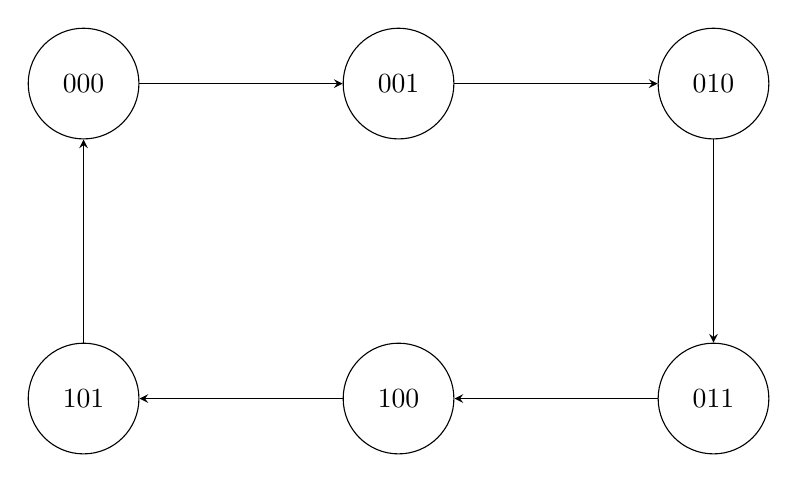
\begin{tikzpicture}[node distance=4cm, on grid, auto, every state/.style={draw, minimum size=4em},>=stealth]
        \node[state] (000) {000};
        \node[state, right=of 000] (001) {001};
        \node[state, right=of 001] (010) {010};
        \node[state, below=of 010] (011) {011};
        \node[state, left=of 011] (100) {100};
        \node[state, left=of 100] (101) {101};

        \path[->]
        (000) edge node {} (001)
        (001) edge node {} (010)
        (010) edge node {} (011)
        (011) edge node {} (100)
        (100) edge node {} (101)
        (101) edge node {} (000);
    \end{tikzpicture}
    \\
    So we can get state transition logic that:\\
    D0 = $\bar{D2}\bar{D1}\bar{D0} + \bar{D2}D1\bar{D0} + D2\bar{D1}\bar{D0}$\\
    D1 = $\bar{D2}\bar{D1}D0 + \bar{D2}D1\bar{D0}$\\
    D2 = $\bar{D2}D1D0 + D2\bar{D1}\bar{D0}$\\
    So we can draw the logic circuit that:\\
    the reset state is:\\
    \includegraphics[width=0.8\textwidth]{hw4_q2_logic_circuit.png}\\
    among it, the output0 is the lsb of the next-state and the output2 is the msb of the next-state\\
    the DFF0 is the lsb of the current-state and the DFF2 is the msb of the current state.\\
\end{answer}

\newpage
\section{Finite state machine}

The function of a vending machine which sells bottles of soda is described below:

\begin{itemize}
    \item[$\bullet$] Each bottle costs \$1.50.
    \item[$\bullet$] The machine only accepts \$0.50 and \$1 coins. If a customer inserts enough coins, the machine will dispense a bottle of soda (FSM will output ``1", otherwise ``0'') and returns change if needed , e.g., the output of DISPENSE states may be ``1 \$0.5", other states' output may be ``0 \$0''.
    \item[$\bullet$] The process happens one coin at a time, and there is no simultaneous insertion of multiple coins or shipping of multiple bottles. After each transaction, the vending machine enters the IDLE state.
    \item[$\bullet$] We don’t need to account for a scenario where a customer inserts coins but decides not to make a purchase.
\end{itemize}


(a) Draw the FSM (Moore machine) for this vending machine.\textbf{[15 pt]}

(b) Draw the FSM (Mealy machine) for this vending machine.\textbf{[10 pt]}

(c) Could Moore machines and Mealy machines be converted into each other to implement the same function? Compare their difference.\textbf{[10 pt]}
\begin{answer}[Question 3]
    \item[(a)]
    We introduce eight bit:input1 and input0 represents the coin inserted by customers(00 == 0*0.5\$ 01 == 1*0.5\$ 10 == 2*0.5\$), output1 represents whether the machine will dispense a bottle of soda and output2 represents whether the machine will return change(it will only be 0\$ or 0.5\$ i.e. the output2 will only be 0 or 1). Moreover, of course, we have currentstate1, currentstate0 and nextstate1, nextstate0 to represents the coins which have been inserted into the machine.\\
    for Moore machine, we introduce currentstate2 and nextstate2, which are the msb of state bits and currentstate0 and nextstate0 are the lsb of the state bits.output1 is the msb of output state bits and output2 is the lsb of the output state bits.\\
    set 000/00 and 00 to be IDLE\\
    2-bit in binary above the line is the input1 and input0, 3-bit in binary is the currentstate and 2-bit in binary behind the 3-bit is the output1 and the ouput2.\\
    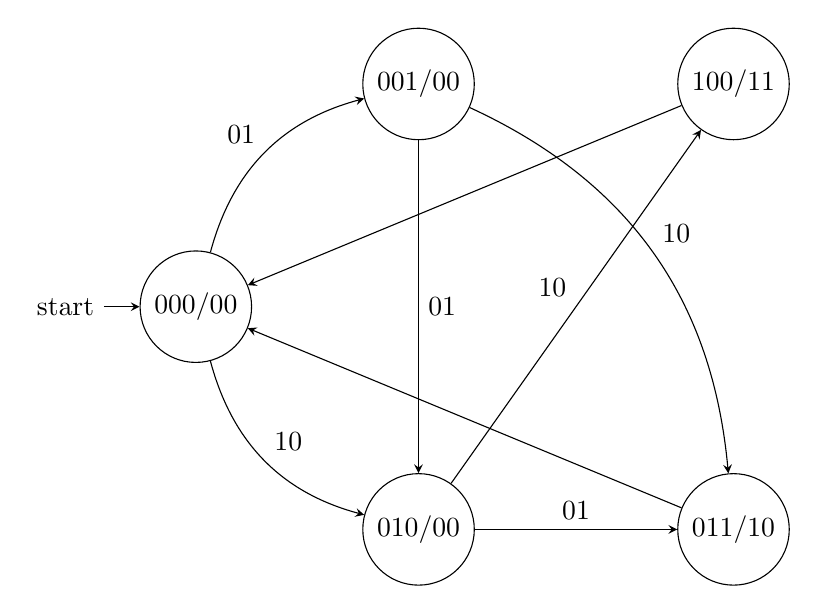
\begin{tikzpicture}[node distance=4cm, on grid, auto, every state/.style={draw, minimum size=4em},>=stealth]
        \node[state, initial] (000/00) {000/00};
        \node[state, above right=of 000/00] (001/00) {001/00};
        \node[state, below right=of 000/00] (010/00) {010/00};
        \node[state, right=of 010/00] (011/10) {011/10};
        \node[state, right=of 001/00] (100/11) {100/11};

        \path[->]
        (000/00) edge[bend left] node {01} (001/00)
        edge[bend right] node {10} (010/00)
        (001/00) edge node {01} (010/00)
        edge[bend left] node {10} (011/10)
        (010/00) edge node {01} (011/10)
        edge node {10} (100/11)
        (011/10) edge node {} (000/00)
        (100/11) edge node {} (000/00);
    \end{tikzpicture}
    \\
    \\
    \\
    \item[(b)]
    for mealy machine, we only use two bits to represnet the currentstate, the 2-bit in binary above the line is the input1 and input0, the other 2-bit in binary hehind the 2-bit is output1 and output2. The 2-bit in binary in the circle is the currentstate1 and the currentstate0.\\
    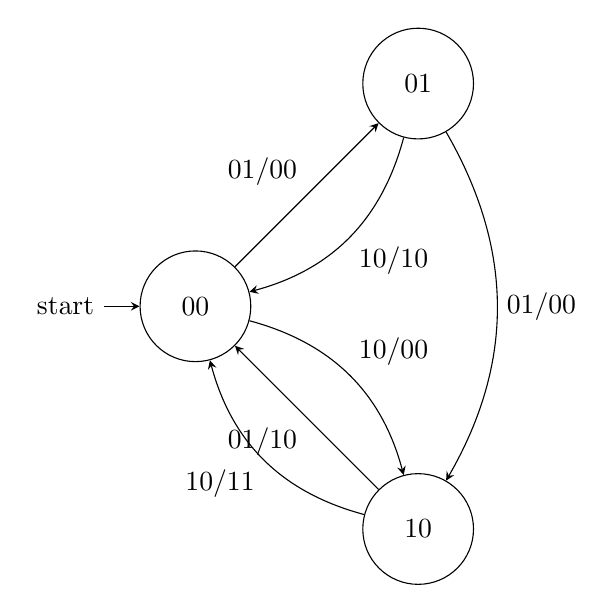
\begin{tikzpicture}[node distance=4cm, on grid, auto, every state/.style={draw, minimum size=4em},>=stealth]
        \node[state, initial] (00) {00};
        \node[state, above right=of 00] (01) {01};
        \node[state, below right=of 00] (10) {10};

        \path[->]
        (00) edge node {01/00} (01)
        edge[bend left] node {10/00} (10)
        (01) edge[bend left] node {01/00} (10)
        edge[bend left] node {10/10} (00)
        (10) edge node {01/10} (00)
        edge[bend left] node {10/11} (00);
    \end{tikzpicture}
    \\
    So, we have the truth table:\\
    \includegraphics[width=0.8\textwidth]{hw4_q3_2_truth_table.png}\\
    Among it, "-"represents such state(and the corresponding currentstate does not exist too) does not exist.(we can not change the currentstate input, so using "-" to represents such situation does not exist)\\
    And according to the truth table, we can draw the Mealy machine by logisim:\\
    \includegraphics[width=0.8\textwidth]{hw4_q3_2_logic_circuit_mealy_FSM.png}\\
    \item[(c)]
    Yes,they can be converted into each other to implement the same function.\\
    Difference:\\
    In a Moore machine, the outputs depend only on the current state of the machine.Outputs are associated with states, meaning each state has a defined output value.The output of a Moore machine changes only when the state changes.\\
    In a Moore machine, the outputs depend only on the current state of the machine.Outputs are associated with state transitions, meaning the output can change as soon as an input is received and a state transition occurs.The output of a Mealy machine can change with each clock cycle or input event, not just when the state changes.\\
    1.Moore machines have deterministic output behavior, as the output is solely determined by the current state while Mealy machines have output behavior that can change more frequently, as outputs depend on both the current state and the input.\\
    2.In Moore machines, the state transition logic defines the next state only, without considering the input while In Mealy machines, the state transition logic defines both the next state and the output based on the input and the current state.\\
    3.Moore machines can be more synchronized as their outputs are updated only when the state changes, typically synchronized to a clock signal while Mealy machines can have outputs that update asynchronously with respect to the state changes, as they can be influenced by the inputs directly.\\
\end{answer}

\end{document}
